%%%%%%%%%%%%%%%%%%%%%%% file proyecto.tex %%%%%%%%%%%%%%%%%%%%%%
%
% Archivo fuente para el proeycto de trabajo de fin de carrera
%
%%%%%%%%%%%%%%%%%%%%%%%%%%%%%%%%%%%%%%%%%%%%%%%%%%%%%%%%%%%%%%%%%%%

% Configuración (para artículo).

% Clase del documento.
\documentclass[runningheads,a4paper,spanish]{llncs}

% Paquetes
\usepackage[utf8]{inputenc}
\usepackage[spanish]{babel}
\usepackage{url}
\usepackage{graphicx}
\usepackage{rotating}
\usepackage{calc}

\graphicspath{{img/}}

\urldef{\correo}\path|hectornvm@gmail.com|
\def\keywordname{{\bf Palabras clave:}}
\newcommand{\pclave}[1]{\par\addvspace\baselineskip
\noindent\keywordname\enspace\ignorespaces\textnormal{#1}}
\addto\captionsspanish{%
\def\bibname{Bibliografía}%
}


\newenvironment{narrow}[2]{%
\begin{list}{}{%
\setlength{\topsep}{0pt}%
\setlength{\leftmargin}{#1}%
\setlength{\rightmargin}{#2}%
\setlength{\listparindent}{\parindent}%
\setlength{\itemindent}{\parindent}%
\setlength{\parsep}{\parskip}}%
\item[]}{\end{list}}





% Cuerpo del documento
\begin{document}

\mainmatter  % start of an individual contribution


\title{Trabajo Fin de Carrera
\\Implantación de un museo virtual en el Real Observatorio de Madrid}
\author{Héctor Navarro Martín}

\authorrunning{Héctor Navarro Martín}
\titlerunning{Museo virtual en el Real Observatorio de Madrid}

% (feature abused for this document to repeat the title also on left hand pages)

\institute{Ingeniería en Informática
\\Escuela Técnica Superior de Ingeniería Informática
\\Universidad de Alcalá
\\\correo}

\date{\today}
\maketitle % Generar el título según la configuración anterior

\pclave{museo virtual, Real Observatorio de Madrid, OAN, IGN, cms, wiki.}


\newpage

\tableofcontents

\newpage

\section*{Baremación de alternativas}
\par Llegados a este punto, nuestro proyecto tiene que empezar a definirse y descartar unas alternativas de otras. Hasta la fecha, recapitulando, hemos puesto encima de la mesa la necesidad de un gestor de contenidos con o sin componente wiki. A este esqueleto inicial habría que añadirle una serie de características y su grado de importancia (donde 0 es prescindible y 5 es imprescindible). Este grado de importancia ha sido recogido en entrevista directa con responsables de la supervisión del proyecto.

\subsection*{Relación de características}

\begin{tabular}{l @{\hspace{10px}} r}
Caracerística & Nota \\
\hline \\
Interfaz de creador en español & 4 \\
Interfaz de usuario en múltiples idiomas & 5 \\	
Varias perspectivas diferenciadas & 1 \\
Web semántica & 0 \\
Uso de estándares & 0 \\
Editor WYSIWYG & 5 \\
Soporte comercial & 1 \\
Comunidad de desarrolladores / soporte & 4 \\
Actualizaciones recientes & 1 \\
Entorno colaborativo & 3 \\
Buzón de sugerencia / Preguntas frecuentes & 0 \\
Página de control de cambios / CVS & 5 \\
Licencia libre & 5 \\
Base de datos & 3 \\
Sistema de ficheros (en contraposición a BD) & 0 \\
Posibilidad de exportar a pdf/LaTeX & 1 \\
Versión para plataformas móviles & 4 \\
Blog & 0 \\
\end{tabular}

\subsection*{Comentarios}

\par La cuestión sobre las perspectivas diferenciadas se ha decidido plantear a la manera de Wikipedia, es decir, a base de enlaces con contenido más exhaustivo en vez de un selector de perspectiva que nos dejase ``ponernos las gafas" de ``estudiante", ``visitante" o ``investigador" con un botón, al menos, en esta fase del proyecto.

\par Aun no habiendo resuelto temas importantes como si la figura del ``responsable de mantenimiento" de la aplicación existirá y quién se encargaría de ella, en la misma reunión se esbozó la idea de que existiría una fase inicial de carga con un principio y un final y una fase de mantenimiento en la que se harán cambios pero a menor ritmo. Todas ellas irán recubiertas de la figura del supervisor, que se encargará de aprobar o rechazar los cambios u añadidos propuestos por los generadores de contenido antes de que éstos se reflejen en la producción final.

\par En contrapartida a las ideas de blog y buzón de sugerencias, se propondrá (con mayor o menor grado de insistencia) al usuario realizar una encuesta evaluación con su propio espacio para sugerencias.

\par El tema de uso de estándares y web semántica, si bien es un objetivo deseable, no debe obstaculizar el resto de ellos, se asume de la última reunión.

\par Por último, y para que la base de datos creada pueda ser fácilmente usada por otros proyectos, se ha optado por buscar una solución orientada a bases de datos y no a sistemas de ficheros como modo de almacenamiento. Esto descartará unas cuantas opciones.

\section*{Comparativa}

\par Habiendo descartado o relativizado la importancia de algunos de los requerimientos iniciales para nuestro gestor de contenidos, vamos a tratar de hacer una propuesta inicial. Para ello, vamos a utilizar herramientas gratuitas en línea que presentan los datos como una matriz de características (CMSMatrix.org y CMSMatch.com).

\subsection*{Premisas iniciales}
\par Las premisas iniciales para los CMS (y las que más descartan) son:

\begin{itemize}
\item Más populares y mejor puntuados. De esta manera potencialmente hayaremos estabilidad y una comunidad de soporte activa. Para ello, echaremos un vistazo a las estadísticas disponibles en la red sobre CMS más utilzados, mejor puntuados y más premiados, tratando de sopesar adecuadamente cada fuente.
\item Editor visual (WYSIWYG Editor / Drag'n'Drop interface).
\item Con capacidad para gestionar la plataforma en varios idomas (Internationalization = Multilingual Content / Multilingual Content Integration / Web-based Translation Management).
\item Página de cambios (Versioning / Asset Management=Media Library)
\item Coste cero.
\item Licencia OpenSource.
\item Comunidad de desarrolladores (Developer Community).
\item Interfaz en español (Interface Localization).
\item Versión para móviles (Mobile Internet).
\end{itemize}

\subsection*{Candidatos pre-seleccionados}
\par Primeros elegidos por su demostrada utilización, premios, etc:

\begin{enumerate}
\item dotCMS
\item Drupal
\item Joomla!
\item LifeRay Portal
\item MODx
\item mojoPortal
\item Moodle
\item Plone
\item SilverStripe
\item WordPress
\end{enumerate}

\par El primer problema que encontramos es que estos sistemas que hemos elegido para comparar los diferentes CMS no nos dejan saber qué idiomas tiene la interfaz de usuario, así que ha que hacer una pequeña investigación entrando en las páginas web de cada uno de los sitios. Tras esto, sabremos que, al menos en cuanto a la interfaz de administración, todas las plataformas preseleccionadas pueden ejecutarse en español.


\par A continuación, pasamos a desgranar las dos comparativas hechas con las diferentes herramientas encontradas:

\subsection{Comparativa con CMSMatrix}

\par En esta ocasión, vamos a ir comparando las características más reseñables de cada producto, por bloques, según está organizado en el servicio consultado.

\subsubsection{System Requeriments (Requisitos de sistema)}

\par Vamos a ir analizando lo que se ve en la figura:

\begin{figure}
\begin{narrow}{-0.2\linewidth}{-0.2\linewidth}
\centering
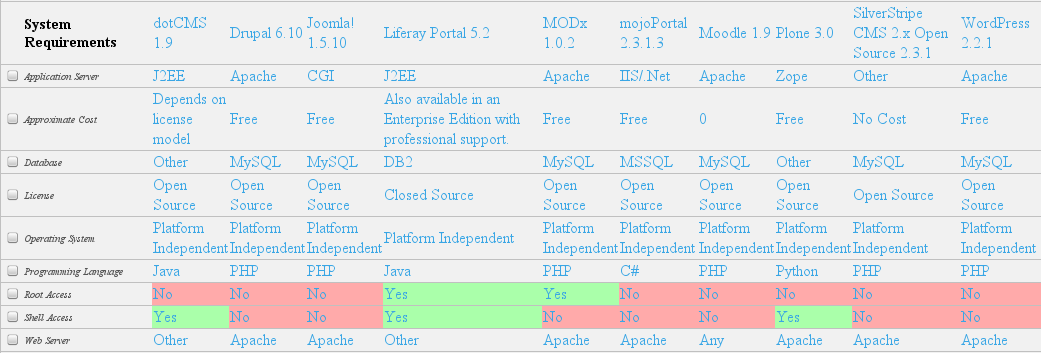
\includegraphics[width=\linewidth]{cmsmat1}
\caption{System Requeriments desde CMSMatrix.org}
\end{narrow}
\label{fig:cmsmat1}
\end{figure}

%\begin{sidewaysfigure}
%  \centering
%   \includegraphics[width=\textheight]{proyecto2}
%\caption{Diagrama de Gantt del proyecto}
%\label{fig:gantt2}
%\end{sidewaysfigure}



\end{document}